\documentclass[12pt]{handout}
\course{Math 1181H}
\author{Jim Fowler}
\geometry{margin=0.5in}
\usepackage{tikz}
\usetikzlibrary{calc}
\include{preamble}
\title{Sums of angles in a triangle}
\usetikzlibrary{patterns}

\begin{document}
\maketitle

\noindent\textbf{What do the three angles of a triangle sum to?}  In
the Euclidean case, you know the answer.

\begin{center}
\begin{tikzpicture}[node distance=1cm]
  \coordinate (a) at (0,0);
  \coordinate (b) at (4,1);
  \coordinate (c) at (2.4,5);
  \coordinate (bc) at ($ (b)!0.5!(c) $);
  \coordinate (ab) at ($ (a)!0.5!(b) $);
  \coordinate (ac) at ($ (a)!0.5!(c) $);

  \draw (a) -- (b) -- (c) -- (a);

%  \node[anchor=north] (label1) at  ($ (a)!0.5!(b) $) {$C$};
%  \node[anchor=west] (label2) at  ($ (b)!0.5!(c) $) {$A$};
%  \node[anchor=east] (label3) at  ($ (c)!0.5!(a) $) {$B$};

    \node[anchor=south west] (labela) at ($ (a)!0.1!(bc) $) {$a$};
    \node[anchor=south east] (labelb) at ($ (b)!0.15!(ac) $) {$b$};
    \node[anchor=north] (labelc) at ($ (c)!0.125!(ab) $) {$c$};

  \node (equation) at (6,2) {$a+b+c = 180^\circ$};

  \clip (a) -- (b) -- (c) -- (a);
  \draw (a) circle (0.5cm);
  \draw (b) circle (0.5cm);
  \draw (c) circle (0.5cm);

\end{tikzpicture}
\end{center}


\textbf{What about in the five-squares-to-a-vertex case?}  Cut out the
following shapes, then cut along the dotted line, attach the tab
labeled \textsf{\textbf{GLUE TO A}} to the square containing vertex
$a$, and attach the tab 
labeled \textsf{\textbf{GLUE TO C}} to the square containing vertex $c$.

\begin{center}
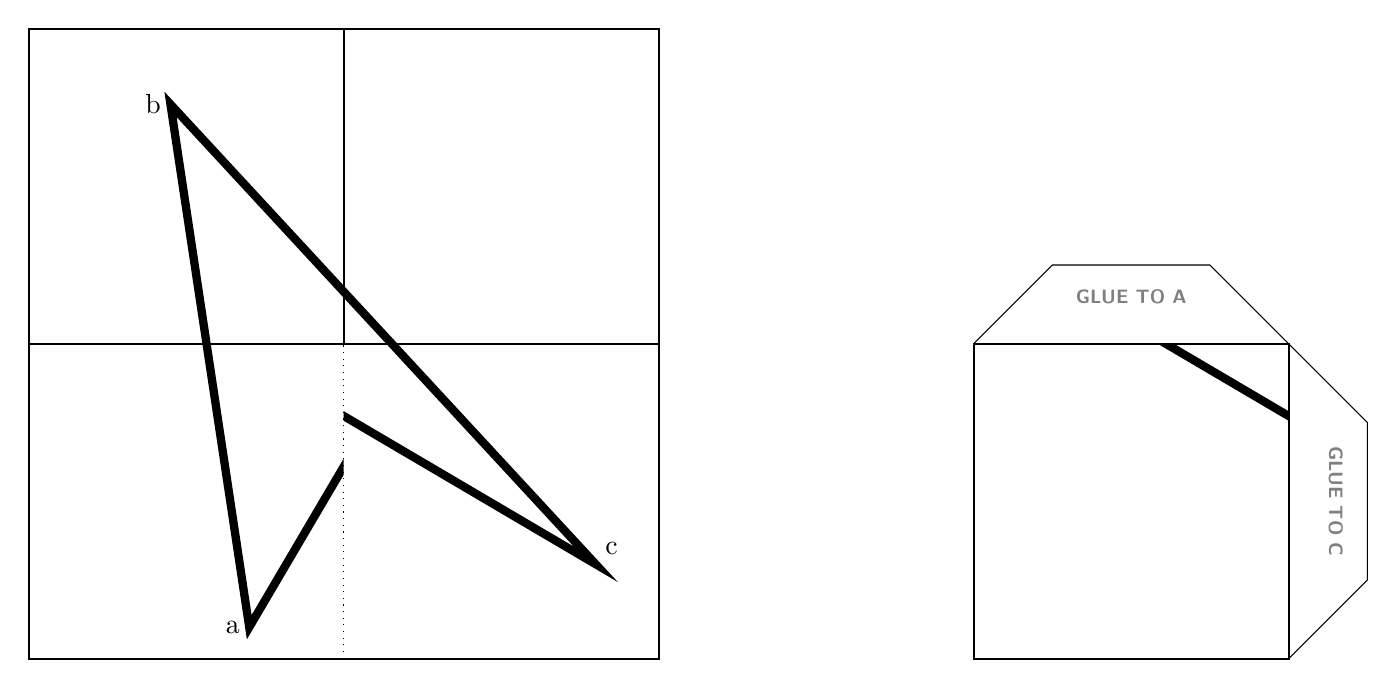
\begin{tikzpicture}[scale=4]

  \draw[thick] (-1,-1) rectangle (1,1);
  \draw[thick] (0,0) -- (0,1);
  \draw[thick] (-1,0) -- (1,0);
  \draw[dotted] (0,-1) -- (0,0);

  \coordinate (a) at (-0.3,-0.9);
  \coordinate (a') at (-0.9,0.3);
  \coordinate (b) at (-0.55,0.76);
  \coordinate (c) at (0.8,-0.7);
  \coordinate (c') at (0.7,0.8);

  \coordinate (ap) at ({3-0.9},{0.3});
  \coordinate (cp) at ({3+0.8},{-0.7});

  \node[anchor=east] (label) at (a) {a};
  \node[anchor=east] (label) at (b) {b};
  \node[anchor=south west] (label) at (c) {c};

  \begin{scope}
    \clip (-1,0) rectangle (1,1);
    \draw[line width=3pt] (a) -- (b) -- (c);
  \end{scope}

  \begin{scope}
    \clip (-1,-1) rectangle (0,0);
    \draw[line width=3pt] (b) -- (a) -- (c');
  \end{scope}

  \begin{scope}
    \clip (0,-1) rectangle (1,0);
    \draw[line width=3pt] (b) -- (c) -- (a');
  \end{scope}

  \draw[thick] (2,-1) rectangle (3,0);
  \begin{scope}
    \clip (2,-1) rectangle (3,0);
    \draw[line width=3pt] (cp) -- (ap);
  \end{scope}

  \begin{scope}[xshift=2cm]
  \draw (0,0) -- (0.25,0.25) -- (0.75,0.25) -- (1,0);
  \node[anchor=center,rotate=0] (label) at (0.5,0.15)
  {\textcolor{white!50!black}{\scriptsize\textsf{\textbf{GLUE TO A}}}};
  \end{scope}

  \begin{scope}[xshift=3cm,rotate=270]
  \draw (0,0) -- (0.25,0.25) -- (0.75,0.25) -- (1,0);
  \node[anchor=center,rotate=270] (label) at (0.5,0.15)
  {\textcolor{white!50!black}{\scriptsize\textsf{\textbf{GLUE TO C}}}};
  \end{scope}

\end{tikzpicture}
\end{center}

\vfill

Here are some questions for you to think about.
\begin{itemize}
\item What do the angles in this example add up to?
\vfill
\item What if you wiggle the points $a$, $b$, and $c$ slightly: how
  does the sum of the angles change?
\vfill
\item What if you draw a much bigger triangle?
\end{itemize}

\vfill

\pagebreak
\null

\end{document}

%%% Local Variables: 
%%% mode: latex
%%% TeX-master: t
%%% End: 
